In this chapter, the case study inside the D-DUST project is explained, paying attention to the data used in the different periods, resolutions and target variables.
\section{Data sets description}
This case study aims to discover the main factors which affect mostly the target variable chosen. 
Variables selected are the physical and chemical factors that are most associated with the formation of primary and secondary pollutants. \newline
Therefore, the variables are categorized into 4 different labels:
\begin{itemize}
\item Weather: these elements, such as wind speed and direction, precipitation and air temperature, change in the epochs and can influence air pollution;
\item Pollutant: these variables represent primary and secondary pollutants related to the greenhouse effect;
\item Soil and Vegetation: since soil and vegetation degradation are global concerns and can influence air propagation in the environment, data related to soil and vegetation characteristics are collected;
\item GIS (time-invariant layers): these time-invariant layers are considered to be changeless in the time range considered. Differently from the other types which need constant monitoring, these variables are updated yearly with a lower frequency than the others;
\end{itemize}
The data chosen are open source and are regularly available.
In this phase, data have been collected (in this repository\footnote{ \url{https://docs.google.com/spreadsheets/d/1-5pwMSc1QlFyC8iIaA-l1fWhWtpqVio2/edit\#gid=91313358}}) in grids from different sources and provided in geopackages. 
\subsection{Source types}
To better distinguish the characteristics of the data sources, the selected variables are labelled with four different types of sources:
\begin{itemize}

\item Ground Sensor: One of the aims of this case study related to the D-DUST project, is to detect the impact on estimates combining data coming from ground sensors to satellite data, and analyse how the local monitoring could improve.  
Each ground monitoring station which provides meteorological and air quality data belongs mainly to: 
\begin{itemize}
    \item ARPA (Agenzia Regionale per la Prevenzione dell'Ambiente);
    \item ESA Air Quality Platform (low-cost sensor) \cite{esasensor};
\end{itemize} 
\begin{comment}
Even if ground sensor measurements have been already validated by ARPA, there were still values out-of-scale. 
To manage this, a supplementary outlier deletion was performed by removing the values that had the absolute value of z score greater than or equal to 4.\\ 
\end{comment}
\item Model: data are estimated through a model built using satellite and meteorological and air quality data as input, such as European data provided by \acrshort{cams};
\item Map layer: this data are time-invariant and are related to Lombardy morphology such as density of roads, population or land use; 
\item Satellite Sensor: They provide data from air quality observation mainly. Satellites providers are Sentinel-5P \acrshort{tropomi} and Terra \& Aqua \acrshort{modis};
\end{itemize}
\bigbreak

In the next lines, each variable is provided in tables, by showing its type, name and description.
\pagebreak
\subsubsection{Meteo Variable (Table)}
\begin{center}
\setlength{\arrayrulewidth}{1.5pt}

\begin{longtable}{ |p{2.1cm}|p{1.4cm}|p{2.7cm}|p{4cm}|p{1cm}|p{2.3cm}| } 
\hline
\textbf{Physical variable} & \textbf{Source type}  & \textbf{Variable name}  & \textbf{Description}  & \textbf{Unit}  & \textbf{Source}\\ 
\hline
\multirow{3}{4em}{Temperature} & Model  & \underline{temp\_2m} & Mean air temperature at 2 m above the land surface.\par & °K & ERA5-Land hourly data.\\ 
& Ground \newline Sensor  & \underline{temp\_lcs} &  Mean air temperature ground measurement - Low-Cost Sensor ESA monitoring stations.\par & °C & ESA Air Quality Platform.\\ 
& Ground \newline Sensor  & \underline{temp\_st} &  Mean temperature - ARPA monitoring stations.\par & °C & ARPA \newline Lombardia.\\ \hline

\multirow{4}{4em}{Wind} & Model  & \underline{e\_wind} & Mean eastward wind component 10 m above the land surface.\par & m/s & ERA5-Land hourly data.\\ 
& Ground \newline Sensor  & \underline{n\_wind} &  Mean northward wind component 10 m above the land surface.\par & m/s & ERA5-Land hourly data.\\
& Ground \newline Sensor  & \underline{wind\_speed\_st} &  Mean wind speed on ground  - ARPA monitoring stations. \par& m/s& ARPA \newline Lombardia.\\ \hline
\pagebreak
\hline
\multirow{2}{4em}{Precipitation} & Model  & \underline{prec} & Mean accumulated liquid and frozen water, including rain and snow, that falls to the Earth's surface. It is the sum of large-scale precipitation. \par & mm & ERA5-Land hourly data.\\ 
& Ground \newline Sensor  & \underline{prec\_st} &  Mean precipitation in each cell in the time range - ARPA monitor stations. \par & mm & ARPA \newline Lombardia.\\ \hline

\multirow{2}{4em}{Air Humidity} & Ground \newline Sensor  & \underline{air\_hum\_st} & Mean air moisture measurement in the time range - ARPA monitoring stations.\par & \% & ARPA \newline Lombardia.\\ 
& Ground \newline Sensor  & \underline{air\_hum\_lcs} &  Mean air moisture ground measurement - Low-Cost Sensor ESA monitoring stations.\par & \% & ESA Air Quality Platform.\\ \hline

\multirow{1}{4em}{Air Pressure} & Model   & \underline{press} & Mean weight of all air in a column vertically above the area of the Earth's surface represented at a fixed point.\par & Pa & ERA5-Land hourly data.\\ \hline

\multirow{1}{4em}{Solar Radiation} & Ground \newline Sensor  & \underline{press} & Global radiation measurement - ARPA monitoring station.\par & W/m\textsuperscript{2} & ARPA \newline Lombardia.\\ \hline

\hline
\caption{Table of Meteorological variables.}

\end{longtable}
\end{center}

\subsubsection{Pollutants Variables (Table)}


\begin{center}
\setlength{\arrayrulewidth}{1.5pt}
\begin{longtable}{ |p{1.6cm}|p{1.5cm}|p{2.3cm}|p{4cm}|p{2cm}|p{2.3cm}| } 
\hline
\textbf{Physical variable} & \textbf{Source type}  & \textbf{Variable name}  & \textbf{Description}  & \textbf{Unit}  & \textbf{Source}\\ 
\hline
\multirow{1}{4em}{Dust} & Model  & \underline{dust} & Mean dust concentration at 0m level provided by CAMS (Ensemble Median - Analysis).\par & $\mu$g/m\textsuperscript{3} & CAMS Model.\\ \hline

\multirow{3}{4em}{AOD} & Satellite \newline Sensor  & \underline{aod\_055} & Mean Aerosol Optical Depth at 550nm.\par & dimension-\newline less & MODIS Terra+Aqua.\\ 
& Satellite \newline Sensor  & \underline{aod\_047} &  Mean Aerosol Optical Depth at 470nm.\par & dimension-\newline less & MODIS Terra+Aqua.\\ 
& Satellite \newline Sensor & \underline{uvai} &  Mean UV Aerosol Index. A positive index highlights the presence of UV-absorbing aerosol (such as smoke/dust). \par & dimension-\newline less & Sentinel-5P\\ \hline
\pagebreak
\hline
\multirow{3}{4em}{PM10} & Model  & \underline{pm10\_cams} & Mean PM10 concentration at 0m level provided by CAMS  (Ensemble Median - Analysis).\par & $\mu$g/m\textsuperscript{3} & CAMS Model.\\ 
& Ground \newline Sensor  & \underline{pm10\_lcs} &  Mean PM10 concentration ground measurement - Low-Cost Sensor ESA monitoring stations.\par & $\mu$g/m\textsuperscript{3} & ESA Air Quality Platform.\\ 
& Ground \newline Sensor & \underline{pm10\_st} &  Mean PM10 concentration ground measurement - ARPA monitoring stations. \par & $\mu$g/m\textsuperscript{3} & ARPA \newline Lombardia\\ \hline

\multirow{3}{4em}{PM2.5} & Model  & \underline{pm25\_cams} & Mean PM2.5 concentration at 0m level provided by CAMS  (Ensemble Median - Analysis).\par &
$\mu$g/m\textsuperscript{3} & CAMS Model.\\ 
& Ground \newline Sensor  & \underline{pm25\_lcs} &  Mean PM2.5 concentration ground measurement - Low-Cost Sensor ESA monitoring stations.\par & $\mu$g/m\textsuperscript{3} & ESA Air Quality Platform.\\ 
& Ground \newline Sensor & \underline{pm25\_st} &  Mean PM2.5 concentration ground measurement - ARPA monitoring stations. \par & $\mu$g/m\textsuperscript{3} & ARPA \newline Lombardia\\ \hline
\pagebreak
\hline
\multirow{3}{4em}{SO\textsubscript{2}} & Model  & \underline{so2\_cams} & Mean SO\textsubscript{2} concentration at 0m level provided by CAMS  (Ensemble Median - Analysis).\par & $\mu$g/m\textsuperscript{3} & CAMS Model.\\ 
& Satellite \newline Sensor  & \underline{so2\_s5p} &  Mean SO2  vertical column density at ground level. \par& mol/m\textsuperscript{2} & Sentinel-5P.\\ 
& Ground \newline Sensor & \underline{so2\_st} &  Mean SO\textsubscript{2} concentration ground measurement - ARPA monitoring stations. \par & $\mu$g/m\textsuperscript{3} & ARPA \newline Lombardia.\\ \hline


\multirow{4}{4em}{NO\textsubscript{2}} & Model  & \underline{no2\_cams} & Mean NO\textsubscript{2} concentration at 0m level provided by CAMS  (Ensemble Median - Analysis).\par & $\mu$g/m\textsuperscript{3} & CAMS Model.\\ 
& Satellite \newline Sensor  & \underline{no2\_s5p} &  Mean NO2  vertical column density at ground level.\par & mol/m\textsuperscript{2} & Sentinel-5P.\\ 
& Ground \newline Sensor & \underline{no2\_st} &  Mean NO\textsubscript{2} concentration ground measurement - ARPA monitoring stations. \par & $\mu$g/m\textsuperscript{3} & ARPA \newline Lombardia.\\ 
& Ground \newline Sensor & \underline{no2\_lcs} &  Mean NO\textsubscript{2} concentration ground measurement - Low-Cost Sensor ESA monitoring stations. \par & $\mu$g/m\textsuperscript{3} & ESA Air Quality Platform.\\ \hline

\multirow{1}{4em}{NO} & Model  & \underline{no2\_cams} & Mean NO concentration at 0m level provided by CAMS  (Ensemble Median - Analysis). \par& $\mu$g/m\textsuperscript{3} & CAMS Model.\\  \hline

\multirow{1}{4em}{CH\textsubscript{2}O} & Satellite \newline Sensor  & \underline{ch20\_s5p} & Mean Formaldehyde tropospheric column number density. \par& mol/m\textsuperscript{2} & Sentinel-5P.\\  \hline

\multirow{1}{4em}{CH\textsubscript{4}} & Satellite \newline Sensor  & \underline{ch20\_s5p} & Mean column averaged dry air mixing ratio of methane. \par& ppbV & Sentinel-5P.\\  \hline

\multirow{1}{4em}{NO\textsubscript{x}} & Ground \newline Sensor & \underline{nox\_st} &  Mean NO\textsubscript{x} (field: "Ossidi di Azoto") concentration ground measurement - ARPA monitoring stations.\par  & $\mu$g/m\textsuperscript{3} & ARPA \newline Lombardia.\\ \hline

\multirow{1}{4em}{CO\textsubscript{2}} & Ground \newline Sensor & \underline{co2\_lcs} &  Mean CO2 concentration ground measurement - Low-Cost Sensor ESA monitoring stations. \par & $\mu$g/m\textsuperscript{3} & ESA Air Quality Platform.\\ \hline
\pagebreak
\hline
\multirow{4}{4em}{CO} & Model  & \underline{co\_cams} & Mean CO concentration at 0m level provided by CAMS  (Ensemble Median - Analysis).\par & $\mu$g/m\textsuperscript{3} & CAMS Model.\\ 
& Satellite \newline Sensor  & \underline{co\_s5p} &  Mean CO vertically integrated column density.\par & mol/m\textsuperscript{2} & Sentinel-5P.\\ 
& Ground \newline Sensor & \underline{co\_st} &  Mean CO concentration ground measurement - ARPA monitoring stations. \par & $\mu$g/m\textsuperscript{3} & ARPA \newline Lombardia.\\ 
& Ground \newline Sensor & \underline{co\_lcs} &  Mean CO concentration ground measurement - Low-Cost Sensor ESA monitoring stations. \par & $\mu$g/m\textsuperscript{3} & ESA Air Quality Platform.\\ \hline

\multirow{3}{4em}{O\textsubscript{3}} & Model  & \underline{o3\_cams} & Mean O\textsubscript{3} concentration at 0m level provided by CAMS  (Ensemble Median - Analysis).\par & $\mu$g/m\textsuperscript{3} & CAMS Model.\\ 
& Satellite \newline Sensor  & \underline{o3\_s5p} &  Mean O\textsubscript{3} total atmospheric column.\par  & mol/m\textsuperscript{2} & Sentinel-5P.\\ 
& Ground \newline Sensor & \underline{o3\_st} &  Mean O\textsubscript{3} concentration ground measurement - ARPA monitoring stations.  \par& $\mu$g/m\textsuperscript{3} & ARPA \newline Lombardia.\\ 
 \hline
 
 \multirow{1}{4em}{CH\textsubscript{2}O}& Satellite \newline Sensor  & \underline{ch20\_s5p} &  Mean Formaldehyde tropospheric column number density. \par & mol/m\textsuperscript{2} & Sentinel-5P.\\ \hline
 
\multirow{1}{4em}{NMVOCs}& Model  & \underline{nmvocs\_cams} & Mean Non-Methane VOCs concentrations at 0m level provided by CAMS.\par & $\mu$g/m\textsuperscript{3} & CAMS Model.\\ \hline

\multirow{3}{4em}{NH\textsubscript{3}} & Model  & \underline{nh3\_cams} & Mean NH\textsubscript{3} concentration at 0m level provided by CAMS  (Ensemble Median - Analysis).\par & $\mu$g/m\textsuperscript{3} & CAMS Model.\\ 
& Satellite \newline Sensor  & \underline{nh3\_lcs} &  Mean NH\textsubscript{3} concentration ground measurement - Low-Cost Sensor ESA monitoring stations. \par  & $\mu$g/m\textsuperscript{3} & ESA Air Quality Platform.\\ 
& Ground \newline Sensor & \underline{nh3\_st} &  Mean NH\textsubscript{3} concentration ground measurement - ARPA monitoring stations. \par & $\mu$g/m\textsuperscript{3} & ARPA \newline Lombardia.\\ \hline
\caption{Table of Pollutant variables.}
\end{longtable}
\end{center}
In addition to them, there are also pollutants variables ending with '\_int' (such as 'pm10\_int', 'pm25\_int', 'nh3\_int', etc.). These variables are obtained by interpolating ARPA variables, which are not spatially continued. The explanation of how they are interpolated and how to mitigate the problem of having a limited number of observations from ground sensors along the surface is in one of the next \hyperref[subsec:nan]{subsection}.
\subsubsection{Soil and Vegetation (Table)}

\begin{center}
\setlength{\arrayrulewidth}{1.5pt}
\begin{longtable}{ |p{2.3cm}|p{1.5cm}|p{2.3cm}|p{4cm}|p{1.3cm}|p{2.5cm}| } 
\hline
\textbf{Physical variable} & \textbf{Source type}  & \textbf{Variable name}  & \textbf{Description}  & \textbf{Unit}  & \textbf{Source}\\ 
\hline

\multirow{3}{4em}{Vegetation} & Satellite \newline Sensor  & \underline{siarlX} & Fraction of area in each cell for each agricultural use provided by SIARL Catalog for Lombardy Region.\par & \% & SIARL Lombardia 2019.\\ 
& Satellite \newline Sensor  & \underline{ndvi} &  Mean NDVI cell value over 16 days period.\par & dimen-\newline sionless & USGS Earth Data.\\ 
& Satellite \newline Sensor  & \underline{siarl} &  Majority class for agricultural use provided by SIARL Catalog for Lombardy Region. \par &catego-\newline rical& SIARL Lombardia 2019.\\
\hline
\pagebreak
\hline
\multirow{5}{4em}{Soil} & Model  & \underline{soil\_moist} & Mean volume of water in soil layer 1 (0 - 7 cm) of the ECMWF Integrated Forecasting System. The surface is at 0 cm. The volumetric soil water is associated with the soil texture (or classification), soil depth, and the underlying groundwater level.\par & m\textsuperscript{3}/m\textsuperscript{3} & ERA5 Land Hourly Data.\\ 
& Map Layer  & \underline{soilX} &  Fraction of area for each cell containing the soil type obtained from OpenLandMap soil texture classification.\par & \% & OpenLandMap Soil Texture Class (USDA System).\\ 
& Map Layer  & \underline{soil\_textX} &  Mean NDVI cell value over 16 days period. \par & \% & Basi informative dei suoli - Geoportale Lombardia.\\ 
& Map Layer  & \underline{soil} &  Majority soil type for each pixel from OpenLandMap soil texture classification .\par &catego-\newline rical& OpenLandMap Soil Texture Class (USDA System) .\\ 
& Map Layer  & \underline{soil\_text} &  Majority soil type for each pixel from Carta pedologica 250K (Lombardy Region). \par&catego-\newline rical& Basi informative dei suoli - Geoportale Lombardia.\\ 

\hline
\caption{Table of variables referred to Vegetation and Soil.}

\end{longtable}
\end{center}

\subsubsection{\acrshort{gis} (static layers) (Table)}
\begin{center}
\setlength{\arrayrulewidth}{1.5pt}
\begin{longtable}{ |p{2.2cm}|p{1.5cm}|p{2.3cm}|p{4cm}|p{2.2cm}|p{2.1cm}| } 
\hline
\textbf{Physical variable} & \textbf{Source type}  & \textbf{Variable name}  & \textbf{Description}  & \textbf{Unit}  & \textbf{Source}\\ 
\hline
\multirow{1}{4em}{Geometry} & Map Layer  & \underline{area} & Area of Lombardy Region vector layer in each cell. \par& km\textsuperscript{2} & \acrshort{siarl} Lombardia 2019.\\ 
\hline
\multirow{1}{4em}{Calendar} & Map Layer  & \underline{cal} & JSON file containing the time-ranges used for data processing. \par& day & -\\ 
\hline

\multirow{1}{4em}{Population} & Map Layer  & \underline{pop} & Population for each cell. & dimensionless& Gridded Population of the World (GPW).\\ \hline

\multirow{2}{4em}{Land use and cover} & Map Layer  & \underline{dsfX} & Land use fraction for each cell containing the classification provided by DUSAF Catalog (Lombardy Region). & \% (fraction for each cell) & DUSAF Lombardia 2018.\\ \hline
Map Layer  & \underline{dusaf} & Cover & Land Use majority class for each cell provided by DUSAF Catalog (Lombardy Region). &categorical & \acrshort{dusaf} Lombardia 2018.\\
\hline
\pagebreak
\hline
\multirow{3}{4em}{Terrain} & Map Layer  & \underline{h\_mean} & DTM average elevation for each pixel. & m & Geoportale Lombardia 2019.\\ 
& Map Layer  & \underline{aspect\_major} & Aspect derived from DTM. Majority pixel aspect. &  °N & Geoportale Lombardia 2019.\\ 
& Map Layer  & \underline{slope\_mean} & Average slope derived from DTM. &  °N& Geoportale Lombardia 2019.\\ 
\hline
\multirow{6}{4em}{Road Infrastru-\newline ctures} & Map Layer  & \underline{int\_prim} & Density of intersection nodes between primary roads for each cell (including highways). & intersections/\newline km\textsuperscript{2} & Geoportale Lombardia 2019.\\ 
& Map Layer  & \underline{int\_prim\_sec} & Density of intersection nodes between primary and secondary roads for each cell. & intersections/\newline km\textsuperscript{2} & Geoportale Lombardia 2019.\\ 
& Map Layer  & \underline{int\_sec} & Density of intersection nodes between secondary roads for each cell. & intersections/\newline km\textsuperscript{2} & Geoportale Lombardia 2019.\\ 
& Map Layer  & \underline{prim\_road} & Density of primary importance roads for Lombardy Region inside for each. & km/km\textsuperscript{2} & Geoportale Lombardia 2019.\\ 
& Map Layer  & \underline{sec\_road} & Density of secondary importance roads for the Lombardy region for each cell. & km/km\textsuperscript{2} & Geoportale Lombardia 2019.\\ 
& Map Layer  & \underline{highway} & Density of highways for Lombardy Region inside for cell divided. & km/km\textsuperscript{2} & Geoportale Lombardia 2019.\\ 
\hline

\multirow{1}{4em}{Farms building} & Map Layer  & \underline{farms} & Fraction of area covered by farms inside the cell. Obtained from DUSAF dataset. & \% (fraction for each cell) & DUSAF Lombardia 2018.\\ \hline
\multirow{1}{4em}{Breeding Farms} & Map Layer  & \underline{farm\_type} & Density of farms classified by breed type for each cell: poultry, pigs, sheeps. & \#farms/km\textsuperscript{2} & DUSAF Lombardia 2018.\\ \hline
\multirow{1}{4em}{Air quality zones} & Map Layer  & \underline{aq\_zone} & Majority class of a given air quality zone in each cell. &categorical & Geoportale Lombardia.\\ \hline
\multirow{1}{4em}{Climate zones} & Map Layer  & \underline{clim\_zone} & Majority class of a given air quality zone in each cell. &categorical& - \\ \hline


\hline
\caption{Table of Static GIS variables.}

\end{longtable}
\end{center}
\pagebreak

\subsubsection{Categorical Variables (table)}
Categorical data are identified with names or labels given to them as value. Even if are represented by numbers, they don't have the same mathematical meaning as a numerical value. 
This type of data is discarded during the pre-processing phase since feature selection is done exclusively on numerical input and output values. \\
The following table explains the semantics of the values assumed.
\bigbreak
\begin{center} 
\setlength{\arrayrulewidth}{1.5pt}
\begin{longtable}{ |p{2.5cm}|p{10cm}| } 
\hline
\textbf{Variable name} & \textbf{Note}\\ 
\hline

 \multicolumn{2}{|c|}{\textbf{Meteo}} \\
\hline
 \underline{wind\_dir\_st}  \newline \newline (Wind direction from ground sensor divided into 8 sectors). & 1 = North: 0° - 22.5° / 337.5° - 360°; \newline2 = North-East: 22.5° - 67.5°; \newline3 = East: 67.5° - 112.5°;  \newline4 = South-East: 112.5° - 157.5°; \newline5 = South: 157.5° - 202.5°; \newline6 = South-West: 202.5° - 247.5°; \newline7 = West: 247.5° - 292.5°; 8 = North-West: 292.5° - 337.5°\\ \hline
 \multicolumn{2}{|c|}{\textbf{Soil and Vegetation}} \\ \hline
 \underline{siarl} \newline \newline (Majority class for agricultural use provided by SIARL Catalog for Lombardy Region). & 2 = Cereal; \newline9 = Mais; \newline12 = Rice;\\  \hline
 \underline{soil} \newline \newline (Majority soil type for each pixel from OpenLandMap soil texture classification). &  1 = Clay; \newline2 = Silty Clay; \newline3 = Sandy Clay; \newline4 = Clay Loam; \newline5 = Silty Clay Loam; \newline6 = Sandy Clay Loam; \newline7 = Loam;\newline8 = Silt Loam; \newline9 = Sandy Loam; \newline10 = Silt; \newline11 = Loamy Sand; \newline12 = Sand;  \\ \hline 
\underline{soil\_text} \newline \newline (Majority soil type for each pixel from Carta pedologica 250K). & 1 = Fine clay;\newline 2 = Very fine clay;\newline  3 = Fine loose;\newline  4 = Coarse loose;\newline  5 = Fine silty;\newline  6 = Coarse silty;\newline  7 = Skeletal-clayey sand;\newline  9 = Skeletal-loose;\newline  10 = skeletal-sand; \\ \hline
 \multicolumn{2}{|c|}{\textbf{GIS (Static layers)}} \\ \hline
 \underline{dusaf} \newline \newline (Land use and cover). & 2 = Agricultural areas; \newline3 = Wooded territories and semi-natural environments; \newline4 = Wetlands; \newline5 = Water bodies; \newline11 = Urbanised areas; \newline12 = Production facilities, large plants and communication networks; \newline13 = Mining areas, landfills, construction sites, waste and abandoned land; \newline14 = Non-agricultural green areas; \\
\hline
 \underline{aq\_zone}\newline \newline (Air quality zones) & 1 = Highly urbanized plains; \newline 2 = Plains; \newline 3 = Prealpi, Appennino and mountains;\newline 4 = Valley floor Agg; 
\newline5 = Urban agglomerated area (Milano, Bergamo, Brescia);\\
\hline
 \underline{clim\_zone}\newline \newline (Climate zones) & 1 = Alpi;\newline 2 = Prealpi Occidentali; \newline 3 = Prealpi Orientali;\newline 4 = Pianura Occidentale;\newline 5 =  Pianura Centrale;\newline 6 = Pianura Orientale; 
 \\
\hline
\caption{Table of categorical variables with their values legend.}



\end{longtable}
\end{center}

To examine the behaviour of each variable in a data set over time, several grid data are collected, each one with a different resolution, period and configuration.
\subsection{Spatial resolution}
Vector grids that are used in the D-DUST project are two and are generated by the spatial resolution of the source provider. 

\begin{itemize}
\item Grids with Copernicus \acrshort{cams} resolution (0.1°); resolution with Copernicus CAMS (European);
\item Grids with 0.01° Grid defined with maximum one \acrshort{arpa} station for each cell;
\end{itemize}

Data are scaled and fit in each spatial resolution grid to better analyze the final output model by considering each of them. 

\par
\subsection{Period}  
Data collected are dated 2021 because they are the most recent and, concerning 2020, those that are not particularly affected by emission reduction caused by lockdown for the COVID-19 pandemic \cite{bontempi2022analysis}. 
\pagebreak
In this case study, grid data were chosen by considering the effect of intensive farming activities, with these particular meteorological conditions:
    \begin{itemize}
        \item To have the right conditions for farming, in the period chosen the terrain shouldn't be frozen (Temperature > 0°C). So I selected data coming from the spring, summer and autumn periods (discarding winter);
        \item For better highlighting the effect of intensive farming activities with the usage of fertilizer and pesticides, which are the main pollution emission factors, weeks with no precipitations were selected;
\end{itemize}
In this way, several grid data were chosen from 5 different weeks over the year:
\begin{itemize}
    \item 24 March - 31 March 2021;
    \item 18 April - 25 April 2021;
    \item 17 July - 24 July 2021;
    \item 3 September - 10 September 2021;
    \item 7 October - 14 October 2021
\end{itemize}

\subsection{Target Variables}
In this case study, the chosen target variables represent the pollution phenomena correlated to intensive farming activities, such as PM25 and ammonia emissions. \\
One of the objectives of this step is to detect the main pollutant factors that contribute further to the training of PM25 or NH3 emissions.\\
PM25 and ammonia (NH3) provided by ARPA sensors are the ones chosen as target variables('pm25\_st' and 'nh3\_st').\\
I chose these measurements because are significant primary pollutants from intensive farming \cite{aneja2008farming}. Moreover, air quality monitoring is traditionally measured by fixed ground-sensor.
\\
ARPA air quality monitoring stations, which are operating 24 hours a day 365 days a year, are periodically checked and subject to maintenance, to ensure proper functioning and reliability.\par
Data covariates are divided between input (X) and output variables (Y). X represents all the variables collected in the previous part, except for the pollutant to be analyzed and modelled (such as PM25 or Ammonia), which is assigned to the Y variable.
\subsection{Mountains}
\label{sub:mountains}
Another important parameter configuration used is to filter or not the cells are covered by mountains or not (climate zone = 1/2/3 of Alps and Prealps). \\ 
In this way, I run an extra test for each resolution in which I include only the grid cells that belong to urban and land areas.
I choose also this different configuration since the focus of the D-DUST project is on the Po Valley, an important area related to agriculture.
Since I assume 2 different resolutions and with the possibility to include or not the mountain zones, I obtained 4 different configurations: 
\par
\begin{itemize}
    \item 10km resolution (0.1°) with all clim\_zone (zone pedoclimatiche);
    \item 10km resolution (0.1°) without Alpes and Prealpes (clim\_zone > 3);
    \item 1km resolution (0.01°) with all clim\_zone (zone pedoclimatiche);
    \item 1km resolution (0.01°) without Alpes and Prealpes (clim\_zone > 3);
\end{itemize}
Their spatial representation is shown in figure \ref{fig:configuration}.
\begin{figure}[H] 
\centering
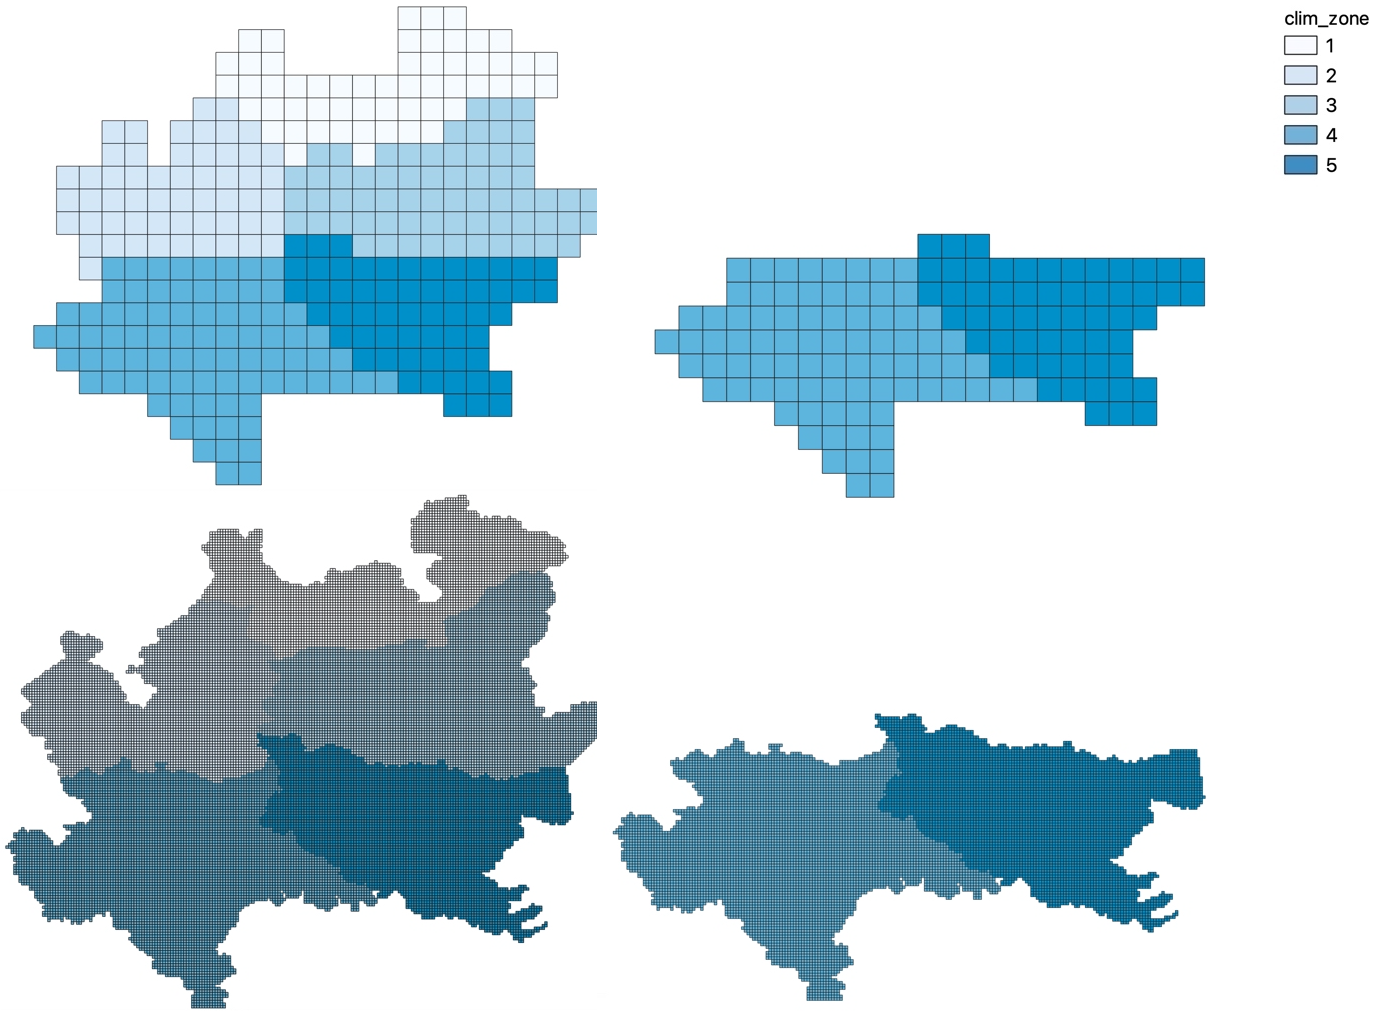
\includegraphics[scale=0.3]{images/configurations.png}
  \caption{Spatial representation of each different test configuration with and without the filter for mountain zones.}
 \label{fig:configuration}
\end{figure}
\section{Data Cleaning of NaN and low-variance values }
\label{subsec:nan}
In my work, I considered as the target variable the PM25 and Ammonia measured by ARPA ground sensors.\\
In the processed grids there is the problem that a given value provided by measurement tools could be NaN. \\
This is caused by the fact that each ground sensor observation, when it is collected in a grid, is assigned to a cell by its location. \\
For this, many cells are not assigned by any ground sensor observations during this step.
So it turns out that variables provided by ARPA and \acrshort{esa} ground sensors (with the label that ends with '\_st' and '\_lcs' respectively) have many NaN cells in the grids in each different resolution (in the figure \ref{fig:knn-interpolated} the only cells containing the values provided by the ground sensors are expressed with the red cross).
\begin{figure}[H] 
\centering
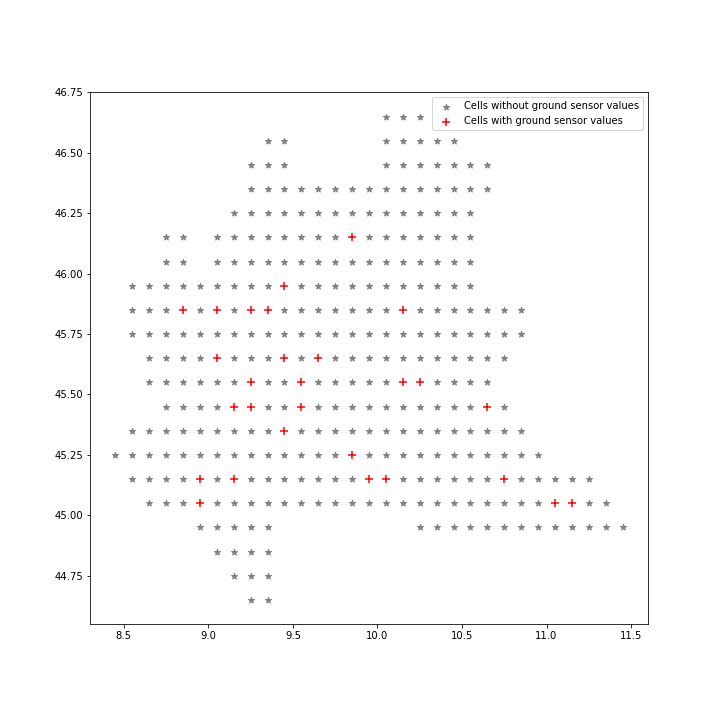
\includegraphics[scale=0.4]{images/cell_with_sensors.png}
  \caption{Graphical representation of the cells which have ground sensor measurements in the grid at 0.1° at resolution.}
 \label{fig:knn-interpolated}
\end{figure}
However, no country in the world has yet established a monitoring network with a fully satisfying coverage \cite{liu2018improve}. Even the United States (US), which is characterized by a relatively developed PM2.5 ground monitoring network with 2500 stations has many areas unmonitored \cite{liu2018improve}. \par
The use of data cleaning produces a data set with several samples too limited to be used for FS or any models.
By seeing figure \ref{fig:cells}, there are respectively only 34 and 8 observations if we considered PM2.5 and Ammonia as target variables.
To mitigate this, I adopted an approach to increase its size with interpolation.
I previously performed a classifier k nearest neighbour \cite{taunk2019brief} to detect the buffer of cells close to the location of the ground station measurement.\\
To increase the number of observations provided by the limited ARPA stations in Lombardy, a k-nearest neighbours algorithm is applied to add the buffer of values (with k, respectively, equal to 10 for 0.1° and 30 for 0.01° resolution). \\ 

\begin{figure}
\begin{multicols}{2}
\begin{verbatim}
****************************
target_variable: 'pm25_st'
resolution = 0.1° (10 km)
old size: 34
new size: 173 
****************************
target_variable: 'pm25_st'
resolution = 0.01° (1 km)
old size: 34
new size: 963 
****************************
****************************
target_variable: 'nh3_st'
resolution = 0.1° (10 km)
old size: 8
new size: 69 
****************************
target_variable: 'nh3_st'
resolution = 0.01° (1 km)
old size: 8
new size: 240 
****************************
\end{verbatim}
\end{multicols}
\caption{In this figure the results of the increment of the number of cells are shown for each different target variable and resolution.}
\label{fig:cells}
\end{figure}

\begin{figure}[H] 
    \centering
    \subfloat[10 km resolution including mountains.]{%
        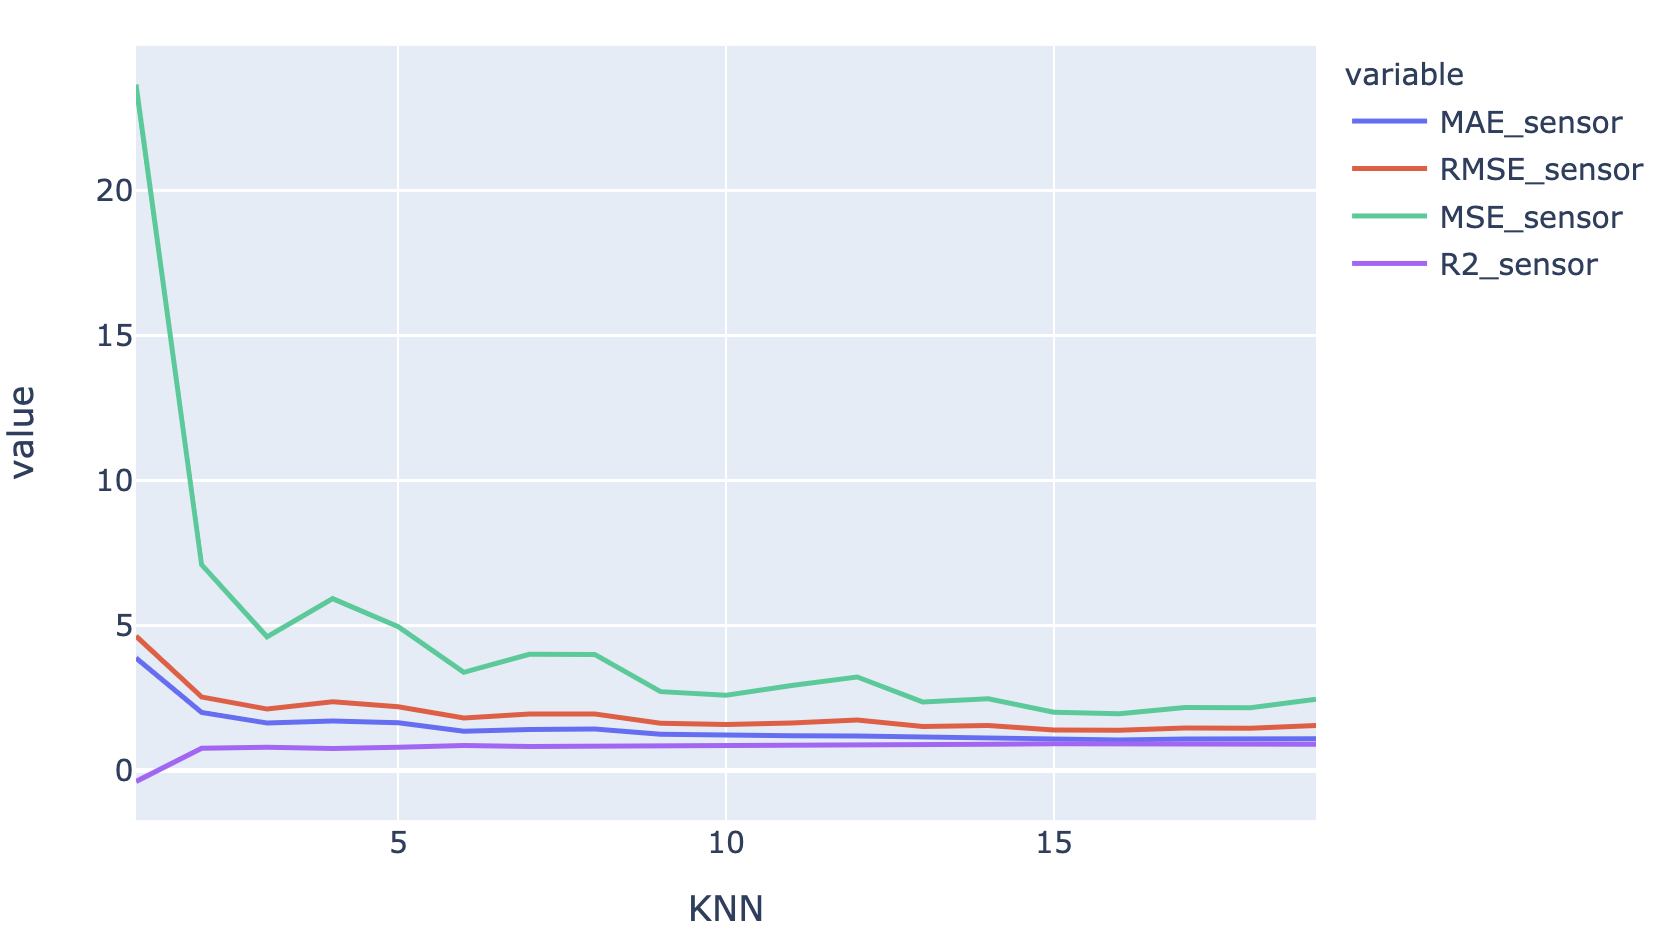
\includegraphics[width=0.55\textwidth]{images/0_1_knn.png}%
        %
        }%
    \hfill%
    \subfloat[1 km resolution including mountains.]{%
        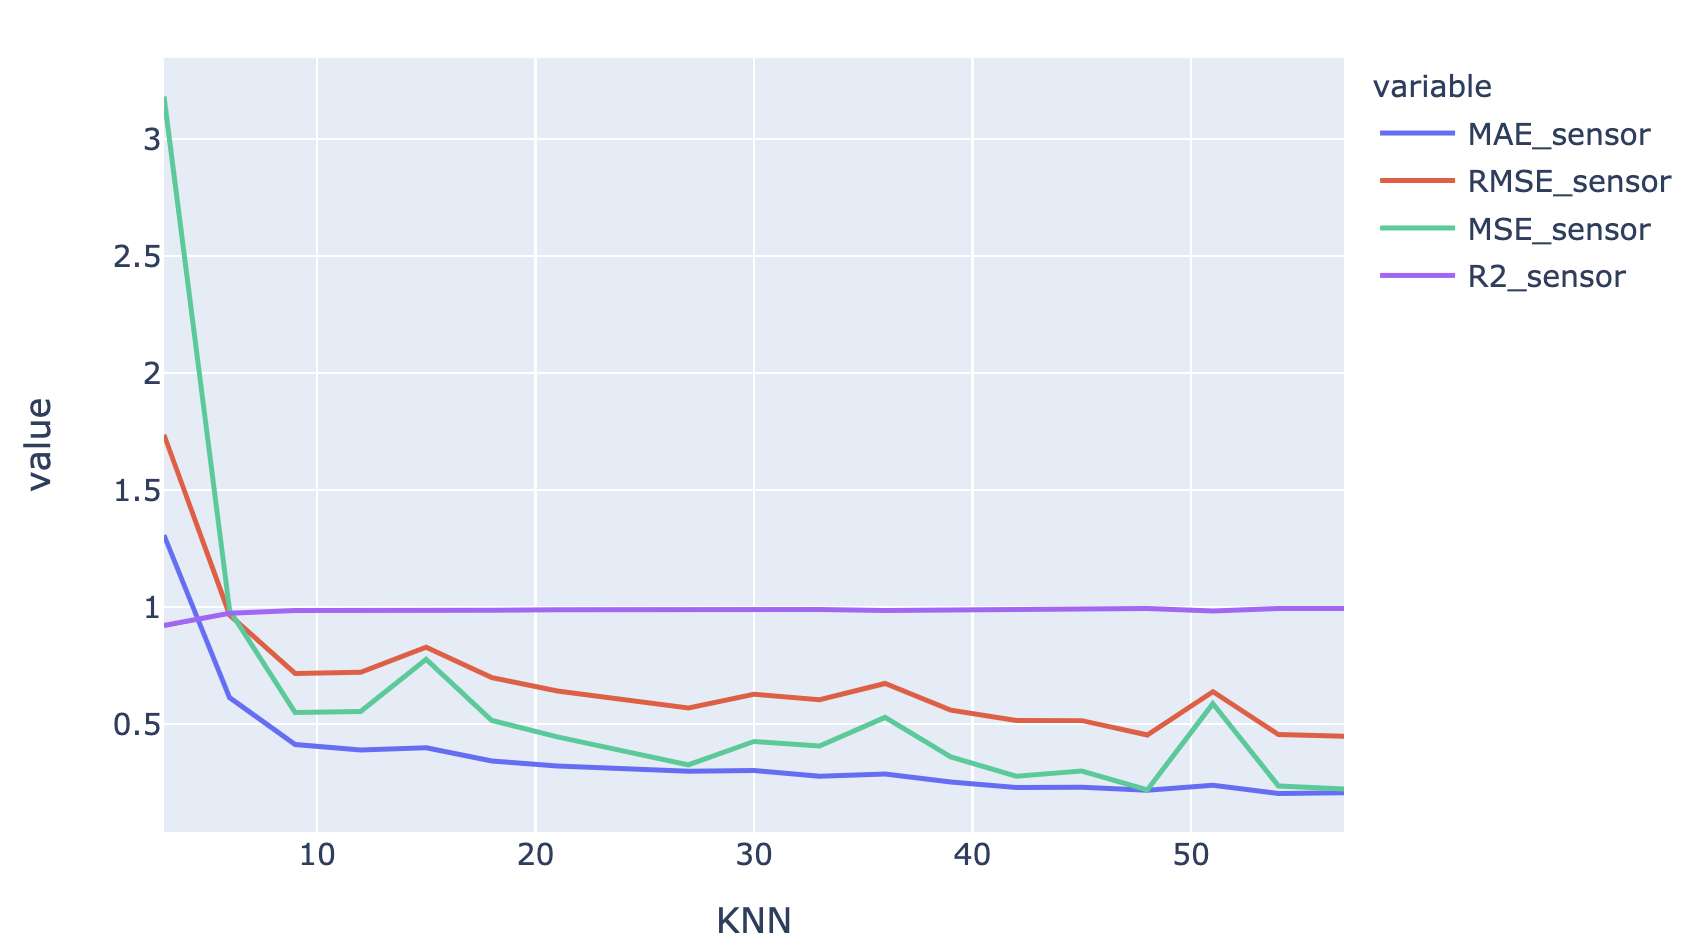
\includegraphics[width=0.55\textwidth]{images/0_01_knn.png}%
        %
        }%
    \caption{Performance in terms of MAE, RMSE, MSE and R\textsuperscript{2} of the Random Forest model with PM2.5 as target variable in function of the K chosen by \acrshort{knn} applied in the data cleaning.}
    \label{fig:knn_chosen}
\end{figure}


\begin{figure}[H] 
    \centering
    \subfloat[PM2.5 as target variable.]{%
        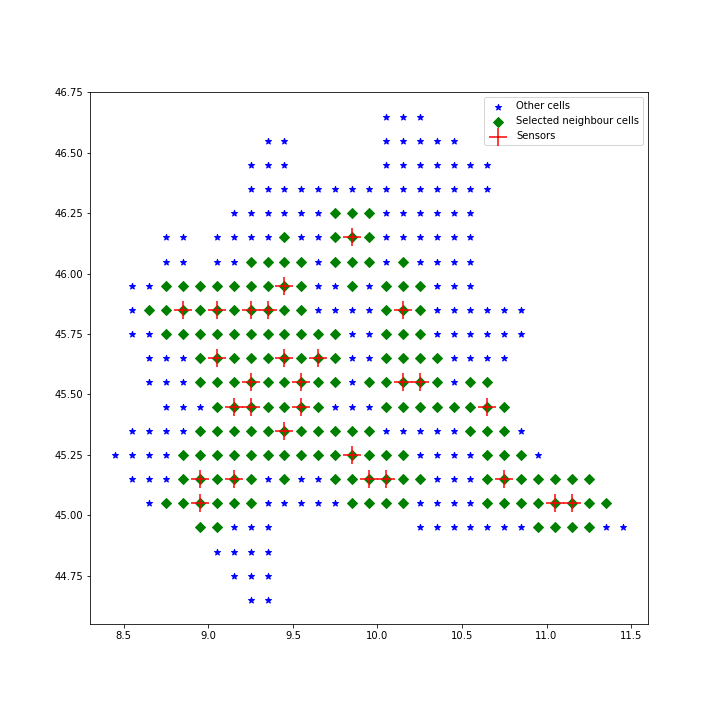
\includegraphics[width=0.5\textwidth]{images/pm25_sensors.png}%
        %
        }%
    \hfill%
    \subfloat[NH3 as target variable.]{%
        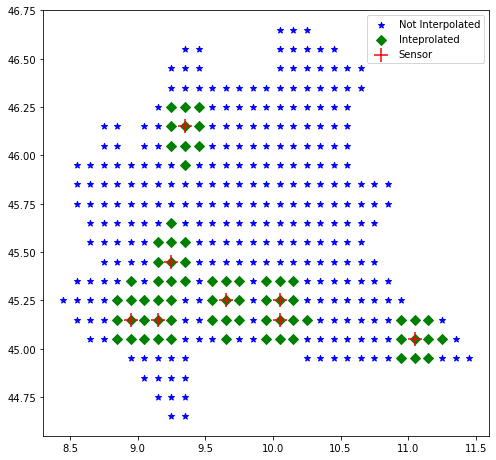
\includegraphics[width=0.5\textwidth]{images/nh3_sensors.png}%
        %
        }%
    \caption{These images show the spatial representation of the cells of the grid data obtained with the use of KNN with 10 km resolution.}
    \label{fig:comparison-sensors1}
\end{figure}
\begin{figure}[H] 
    \centering
    \subfloat[PM2.5 as target variable.]{%
        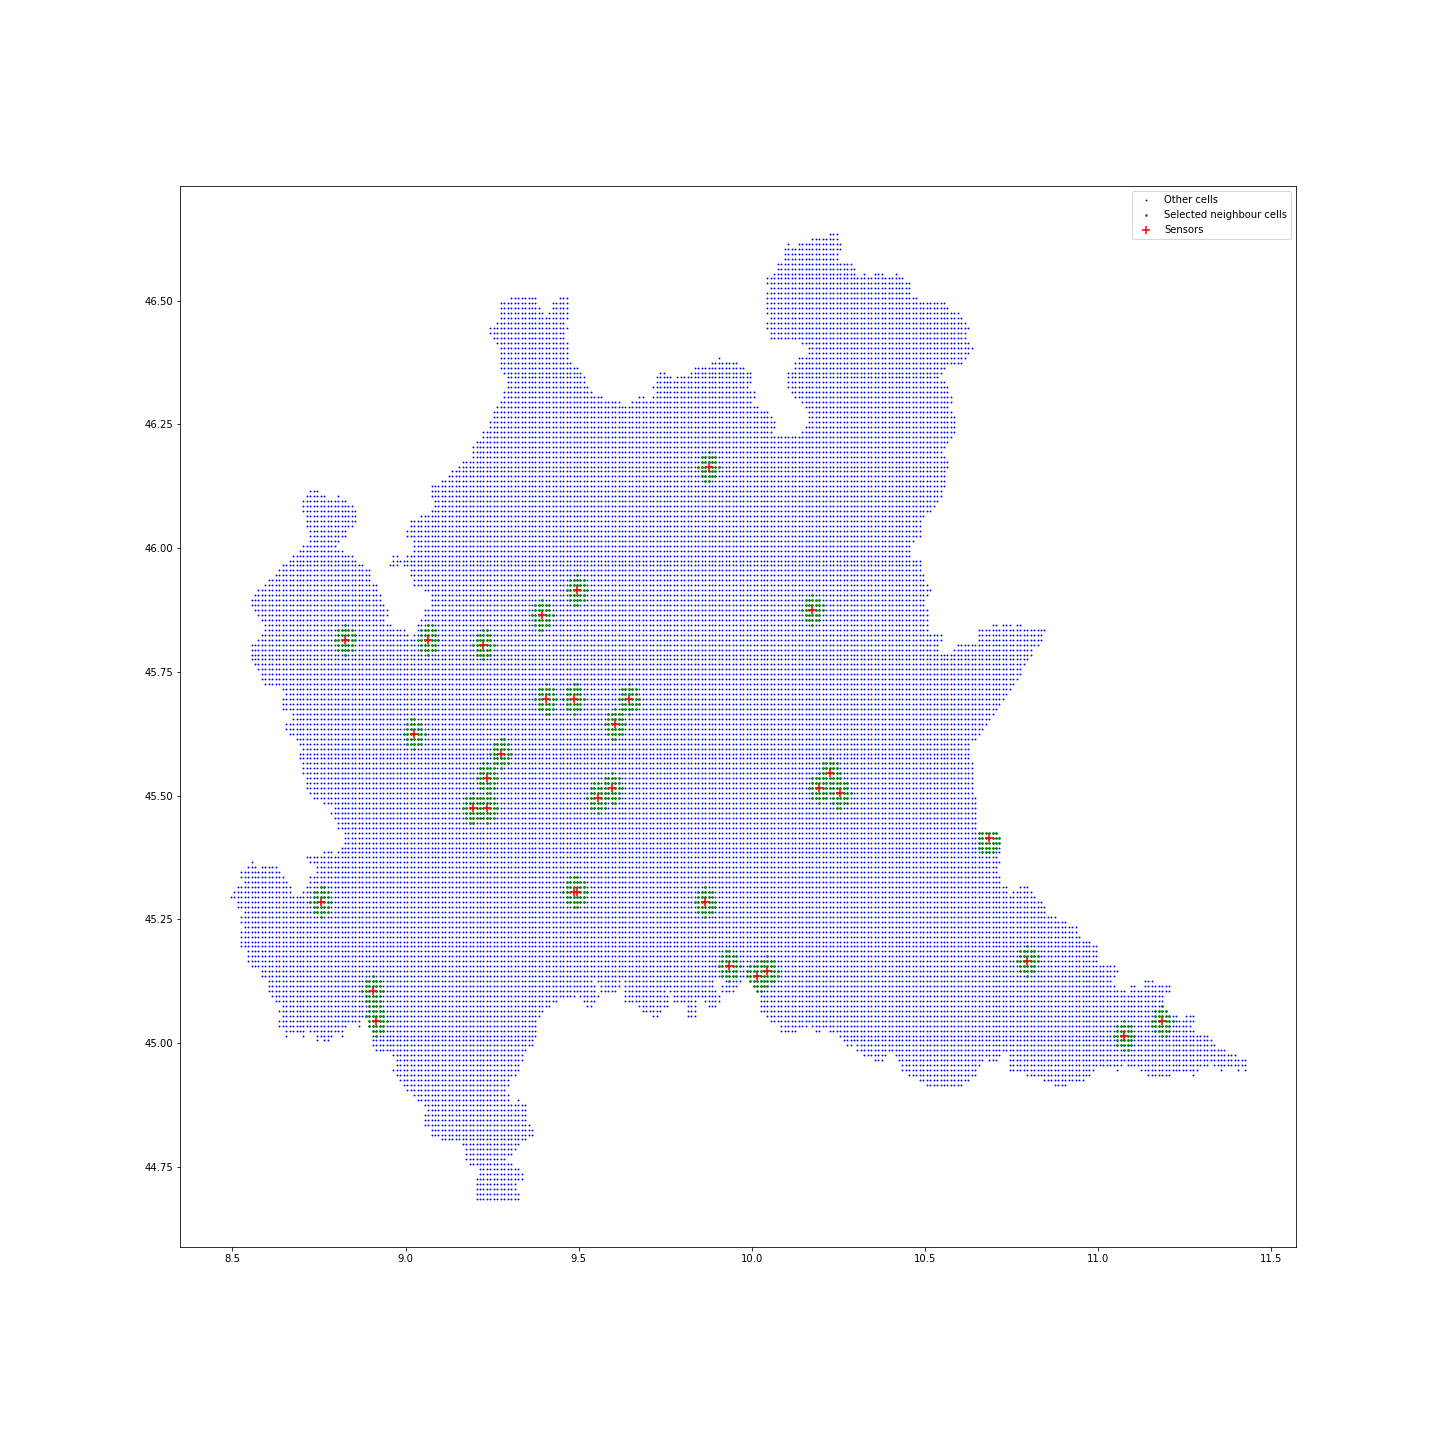
\includegraphics[width=0.5\textwidth]{images/pm25_sensors_1km.png}%
        %
        }%
    \hfill%
    \subfloat[NH3 as target variable.]{%
        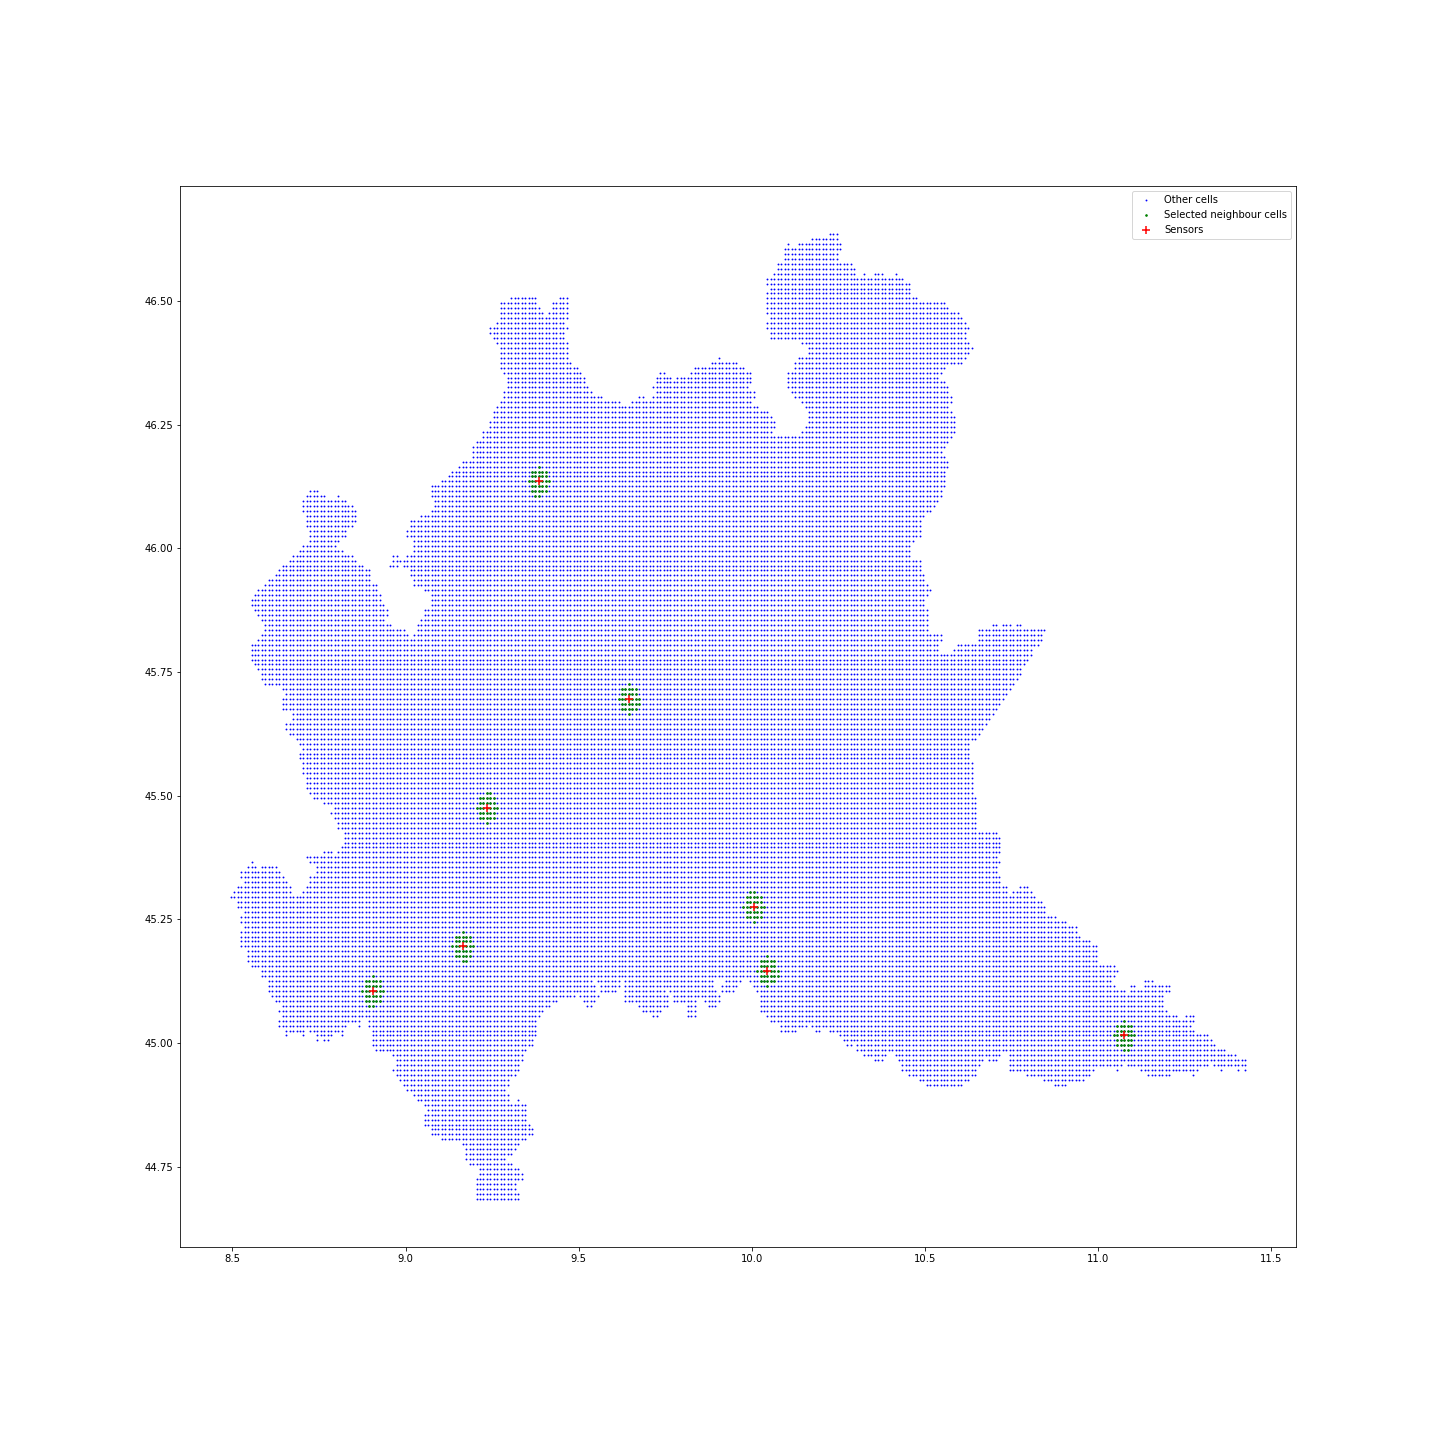
\includegraphics[width=0.5\textwidth]{images/nh3_sensors_1km.png}%
        %
        }%
    \caption{These images show the spatial representation of the cells of the grid data obtained with the use of KNN with 1 km resolution.}
    \label{fig:comparison-sensors2}
\end{figure}
\begin{figure}[H]
\centering
    \includegraphics[scale=0.30]{images/time}
    \caption{Plot of the time spent running KNN algorithm in function of the value of K chosen.}
    \label{fig:time_knn}
\end{figure}



Then, these cells are set with values computed using a \gls{rbf} \cite{wright2003radial} which are separately stored in variables with the name that ends with '\_int'. RBF was performed using linear interpolation.\\
The given procedure is available on GitHub\footnote{\url{https://github.com/gisgeolab/D-DUST/blob/WP2/Ground\%20Sensor\%20Variables\%20Request\%20.ipynb}}.
This approach was not adequately justified because is used only to increase the size of cells with ground sensor measurements for making applicable the FS procedure.
The K chosen used to increase the number of cells with a value is given by a trade-off between the dimension of K and both the accuracy reached by prediction models and the processing time of the KNN algorithm.
Accuracy could be seen in the figure \ref{fig:knn_chosen} where the error metrics of the Random Forest model (described in the next section \ref{sec:modelling}) are in function of the k choosen.
Therefore, for 10 km resolution, I used a K value that allow me to increase partially the number of cells for FS and the model, without increment, particularly the performance. 
In figure TODO the processing time taken to run this method for resolution at 1 km depending on the K chosen is shown.
For 1 km resolution, I chose a K value which allows me to have a minimal increment about the space covered by each cell. Indeed, using a K proportional to the one used at 10 km resolution, the time spent running the algorithms tends to be too high.    
In addition, the values of K for each resolution chosen bring 2 different spatial extensions that could be useful to have differences in the tests executed. The increment of the cells in the grids with 1 km resolution is shown in the figures \ref{fig:comparison-sensors2}

Before the feature selection phase, I removed variables with low variance.
A feature with low variance is characterized by having observations very close to the mean value and thus almost constant.
Features with constant values should be discarded because of their low variability.
In this study \cite{kuhn2008building}, this was performed with a method called nearZeroVar from \gls{caret}, a package in R.
As suggested by this study, I discarded variables which have the following parameters: 
\begin{itemize}
    \item the percentage of unique values greater than 20\%;
    \item the ratio of the most prevalent over the second most prevalent value greater than 20;
\end{itemize} 
This choice in the article is made because of the presence of a very frequent value. This was applied also in this case study due to the presence of many variables related to the fractional land use (such as siarlX and dsfX) which assign 0 to most of the cells. 

\pagebreak
\section{Feature Selection}
In this phase, I computed the FS in tests with different parametrizations.
It can be observed that there are 2 resolutions, and 5 periods. In addition, tests are also executed with and without the mountain zones. Therefore, for each different target variable, (2x5) + (2x5) = 20 different tests were run for both ammonia and fine particulate (thus 20*2 = 40 in total). \\
The \ref{fig:test_params} provide an overview of the different parameters that can be chosen in each test executed depending on the period, resolution, target variable and climate zones chosen.
In the end, the set of FS results of different periods in each configuration is averaged through Borda Count again. An overview of how the results for each different configuration are provided is shown in figure \ref{fig:overview_configuration}.
Thus, in total, this work provided the results for each configuration (4) and target variable (2).
In total in this work are attached 8 (4x2) different results. Each result will be in detail pointed out in chapter \ref{chap:res} and the final Appendix \ref{chap:appendix}.
\begin{figure}[H]
    \centering
    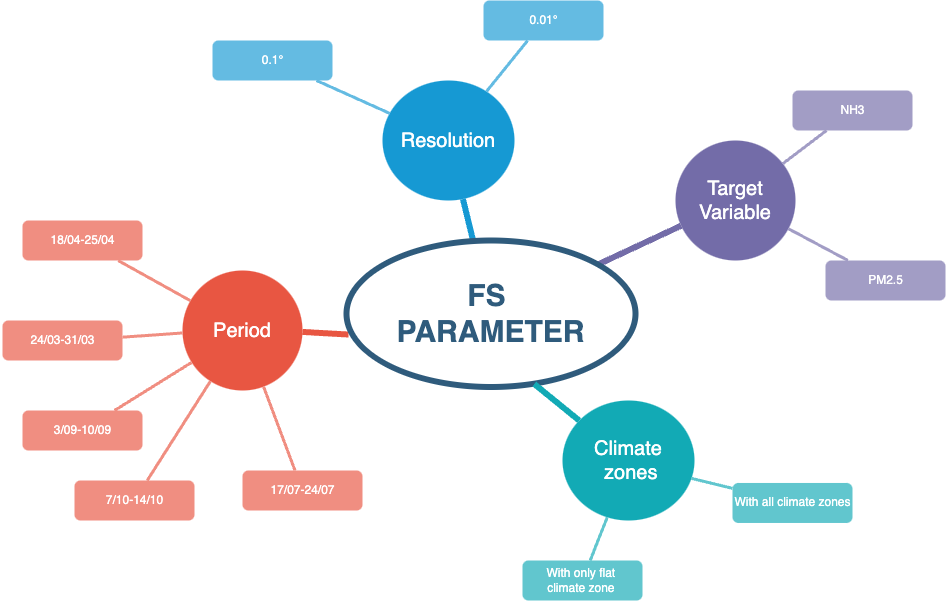
\includegraphics[width=.9\textwidth]{images/test_param.png}
    \caption{Parameter considered for tests execution.}
    \label{fig:test_params}
\end{figure}
\pagebreak

\begin{figure}[H]
    \centering
    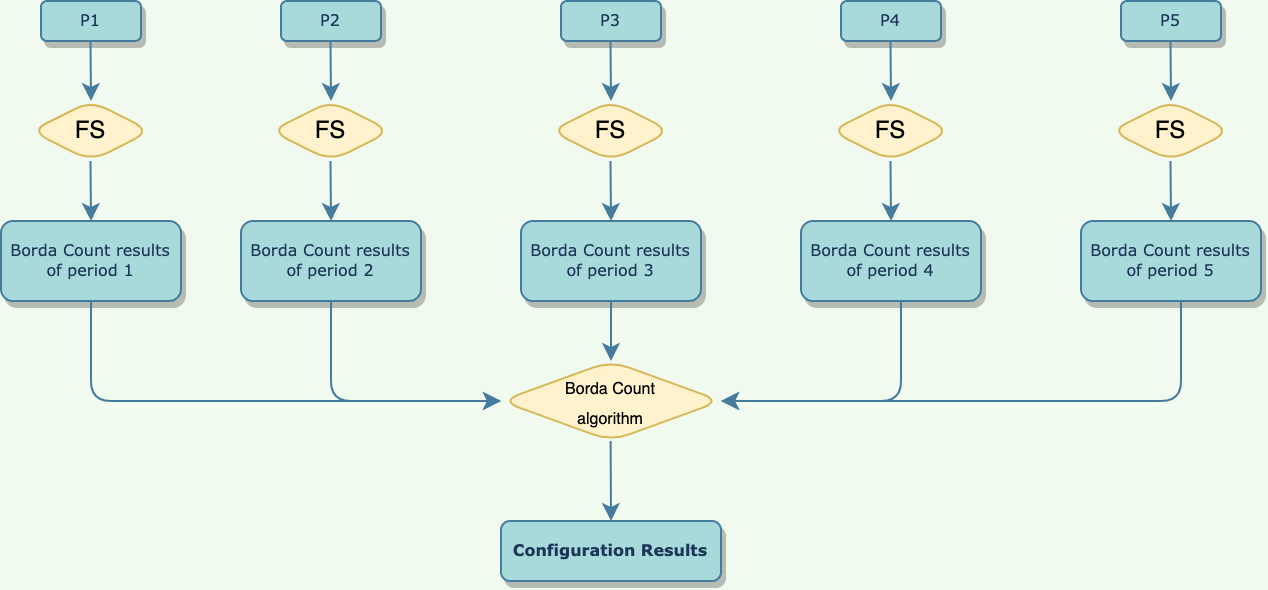
\includegraphics[width=.9\textwidth]{images/overview_results_configuration.png}
    \caption{The following diagram aims to visualize how the results for each different configuration are computed with FS.}
    \label{fig:overview_configuration}
\end{figure}

\pagebreak
\section{Data Modelling}
\label{sec:modelling}
In this phase, I evaluate models trained by the variable selected by \acrshort{fs} to analyze their performance.\\
In detail, the tests run are built and validated using k-fold cross-validation (k=5) which is one of the most used procedures for the evaluation of model performance.\\
I used a 5-fold since brings better performances from some studies in literature \cite{anguita2005k} \cite{jung2020evaluation}.
I perform tests in 2 different ways, explained in the next subsections.
\subsection{Test for different grid}
The validation in each model was made with the values of the target variable (ARPA measurements);
This was applied for each grid data set obtained by the combinations of 4 configurations, 5 periods and 2 target variables (4x5x2 = 40 different model tests). 
In addition, another validation was performed with values assumed by the CAMS model.
Such a procedure was applied to compare the performance of the CAMS model to the current one (results are provided in the appendix \ref{chap:appendixCAMS}).\\
In this way, a comparison between results from these 2 different validations is performed, aiming to detect how much the models perform better in this local scale.\\
These additional results are shown in the appendix \ref{chap:appendix}. 

\subsection{Test for analysing FS impact on performance}
To evaluate how Feature Selection effectively improves the accuracy of the model, a set of tests are run and configured differently from the previous.\\ 
Data from different periods were merged to develop the model through a temporal hold-out validation, where the data are used in this way:
\begin{itemize}
    \item grid data from March, April and July, September periods were used for training;
    \item grid data from the October period was used for validation;
\end{itemize}
In this way, model performance should be evaluated employing external data, which comes from another period.\\
However, before running this, I have to deal with the multicollinearity problem, which can cause bias in the accuracy estimation.\\ 
In the covariates used by both FS and models, there would be variables which could be statistically correlated to others. 
The interdependence of variables would cause unstable estimation, so I tried to solve this issue in these tests.\\ 
To mitigate this, I performed a feature cluster, grouping collinear variables between them. I considered a variable to be collinear to another if and only if the Pearson correlation index is greater than or equal to 0.8, as a study suggests \cite{shrestha2020detecting}. \\
After that, I transformed each cluster of variables using the first \gls{pca} component (called 'PC\_0' component below). In this way, I solved collinearity in the independent variables, without particularly losing the features' interpretability.\\
The groups of variables averaged with PCA are shown in figure \ref{pca01} and \ref{pca001}, where are indicated the groups of collinear variables with the total variance that each PCA component explains. \\
At the end of the figures are shown the new covariates used by the Feature Selection and by RF models, for 10 km and 1 km resolutions, including mountain zones and considering PM2.5 as the target variable.
I grouped and illustrated collinear variables in clusters with the help of a python script\footnote{\url{https://www.kaggle.com/code/nassehkhodaie/fixing-multicollinearity-by-feature-clustering/data?select=collinearity_finder_treater_py.py}}.
\subsubsection{Resolution = 10 km}
\begin{figure}[H]
\begin{verbatim}
**********
cluster_0
variable name = 'dsf2', 'dsf3', 'press'
explained variance by PC_0 = 0.89
**********
cluster_1
variable name = 'dsf14', 'dsf11', 'pop', 'sec_road', 'int_sec', 'dsf12'
explained variance by PC_0 = 0.83
**********
cluster_2
variable name = 'prim_road', 'int_prim_sec'
explained variance by PC_0 = 0.90
**********
cluster_3
variable name = 'nh3_cams', 'siarl9', 'farms'
explained variance by PC_0 = 0.88
**********
cluster_4
variable name = 'o3_s5p', 'uvai'
explained variance by PC_0 = 0.94
**********
cluster_5
variable name = 'nmvocs_cams', 'pm10_int', 'pm10_cams',    
                'no2_cams', 'no_cams', 'pm25_cams', 'co_cams'
explained variance by PC_0 = 0.75
**********
cluster_6
variable name = 'no2_int', 'nox_int'
explained variance by PC_0 = 0.98
**********
cluster_7
variable name = 'o3_cams', 'o3_int'
explained variance by PC_0 = 0.97
**********
cluster_8
variable name = 'temp_int', 'temp_2m'
explained variance by PC_0 = 0.98

New variables: ['dsf5', 'dsf13', 'soil7', 'soil_text3', 'soil_text4', 'farm_pigs',
       'farm_poultry', 'farm_sheep', 'ndvi', 'prec', 'n_wind', 'e_wind',
       'soil_moist', 'aod_047', 'co_s5p', 'dust_cams', 'so2_cams', 'co_int',
       'nh3_int', 'so2_int', 'air_hum_int', 'prec_int', 'rad_glob_int',
       'wind_speed_int', 'cluster_0_pc0', 'cluster_1_pc0', 'cluster_2_pc0',
       'cluster_3_pc0', 'cluster_4_pc0', 'cluster_5_pc0', 'cluster_6_pc0',
       'cluster_7_pc0', 'cluster_8_pc0']
\end{verbatim}
\caption{New features obtained with PCA with 10 km resolution.}
\label{pca01}
\end{figure}
\pagebreak
\subsubsection{Resolution = 1 km}

\begin{figure}[H]
\begin{verbatim}
**********
cluster_0
variable name = 'h_mean', 'slope_mean'

explained variance by PC_0 = 0.9343247371259237
**********
cluster_1
variable name = 'uvai', 'o3_s5p'

explained variance by PC_0 = 0.9502248817971359
**********
cluster_2
variable name = 'nmvocs_cams', 'no_cams', 'no2_cams',
                'pm10_int', 'co_cams', 'pm10_cams', 'pm25_cams'

explained variance by PC_0 = 0.7356224143251505
**********
cluster_3
variable name = 'no2_int', 'nox_int'

explained variance by PC_0 = 0.9760779670033077
**********
cluster_4
variable name = 'o3_cams', 'o3_int'

explained variance by PC_0 = 0.9678067765212931
**********
cluster_5
variable name = 'temp_int', 'temp_2m'

explained variance by PC_0 = 0.9726802610839925
New variables:  ['aspect_major', 'pop', 'dsf2', 'dsf11', 'dsf12', 'soil_text3',
       'soil_text4', 'soil_text9', 'sec_road', 'ndvi', 'prec', 'press',
       'n_wind', 'e_wind', 'soil_moist', 'aod_047', 'co_s5p', 'nh3_cams',
       'dust_cams', 'so2_cams', 'co_int', 'nh3_int', 'so2_int', 'air_hum_int',
       'rad_glob_int', 'wind_speed_int', 'cluster_0_pc0', 'cluster_1_pc0',
       'cluster_2_pc0', 'cluster_3_pc0', 'cluster_4_pc0', 'cluster_5_pc0']
\end{verbatim}
\caption{New features obtained with PCA with 1 km resolution.}
\label{pca001}
\end{figure}